\documentclass{standalone}
\usepackage[rgb]{xcolor}
\usepackage{tikz}
\usepackage{pgfplots}
\usepackage{pgfplotstable}
\usepackage{../mystyle}
\usetikzlibrary{calc}
\pgfplotsset{compat=1.14}

\definecolor{hred}{HTML}{e94b3c}

\begin{document}
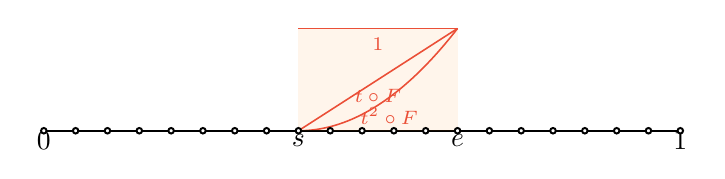
\begin{tikzpicture}
        \begin{axis}[   hide axis,
        					  % only scale the axis, not the axis including the ticks and labels
        						scale only axis=true,
        					 % set `width' and `height' to the desired values
        						width=0.8\textwidth,
                                height=0.15\textwidth,
                                enlarge y limits=0.2
        ]
                        \addplot+[domain=.40:.65, line width=0.2mm, smooth, no marks, hred, opacity=1, solid] {1} node[pos=0.5,anchor=north]{\scriptsize $1$};
                        \addplot+[domain=.40:.65, line width=0.2mm, smooth, no marks, hred, opacity=1, solid] {(x-.4)/(.65-.4)} node[pos=0.5,anchor=north]{\scriptsize $t\circ F$};
                        \addplot+[domain=.40:.65, line width=0.2mm, smooth, no marks, hred, opacity=1, solid] {(x-.4)/(.65-.4)*(x-.4)/(.65-.4)} node[pos=0.35,anchor=north]{\scriptsize $t^2\circ F$};
                        \addplot+[mark=*,mark options={fill=white},mark size=1, color=black, solid, line width=0.25mm] plot coordinates {
                            (0,    0)
                            (1.0/20,   0)
                            (2.0/20,   0)
                            (3.0/20,    0)
                            (4.0/20,    0)
                            (5.0/20,    0)
                            (6.0/20,    0)
                            (7.0/20,    0)
                            (8.0/20,    0)
                            (9.0/20,    0)
                            (10.0/20,    0)
                            (11.0/20,   0)
                            (12.0/20,   0)
                            (13.0/20,    0)
                            (14.0/20,    0)
                            (15.0/20,    0)
                            (16.0/20,    0)
                            (17.0/20,    0)
                            (18.0/20,    0)
                            (19.0/20,    0)
                            (20.0/20,    0)};
                        \draw [fill=orange, opacity = .08,draw=none] (.4,0) rectangle (.65,1) ;
                        \node at (.4,-.1) {$s$};
                        \node at (.65,-.1) {$e$};
                        \node at (.0,-.1) {$0$};
                        \node at (1.,-.1) {$1$};
        \end{axis}
\end{tikzpicture}
\end{document}